\startAnhang

\listofanhang
\clearpage
\anhang{Komplexität von Home Pages}\label{anhang:complexity}
\begin{figure}[htbp]
  \centering
  \includegraphics[width=0.9\textwidth]{graphics/Complexität.png}
  \caption[Komplexität von Home Pages (6 Jahre)]{Entwicklung der Komplexität von Home Pages in den letzten sechs Jahren. Die X-Achse zeigt die Jahre, die Y-Achse gibt die Anzahl der Elemente an.\footcite[Entnommen aus][]{WebAIM}}
  \label{fig:complexity}
\end{figure}

\clearpage

\anhang{Erweiterte Konzeptmatrix}\label{app:konzeptmatrix}
\begin{table}[htbp]
\centering
\setlength{\tabcolsep}{2.5pt}
\renewcommand{\arraystretch}{1.25}

\resizebox{\textwidth}{!}{%
\begin{tabular}{|A|S||*{14}{C|}}
\hline
\multicolumn{2}{|c||}{\textbf{Studie}} &
\multicolumn{14}{c|}{\textbf{Konzepte}} \\
\hline

\multirow{2}{*}{\lhdr{4.3cm}{Autor(en)\\\& Jahr}} &
\multirow{2}{*}{\lhdr{2.8cm}{System}} &
\multicolumn{3}{c|}{\textbf{Ziel}} &
\multicolumn{3}{c|}{\textbf{Datenquellen}} &
\multicolumn{3}{c|}{\textbf{KI-/LLM-Ansatz}} &
\multicolumn{3}{c|}{\textbf{Evaluation}} &
\multicolumn{2}{c|}{\textbf{Kontext}} \\
\cline{3-16}

& &
\hdr{WCAG-Konf.\ prüfen} &
\hdr{Barrieren korrigieren} &
\hdr{Entwickler unterstützen} &
\hdr{Tool-Reports (axe etc.)} &
\hdr{Interaktionsdaten (Playwright)} &
\hdr{Quellcode-Analyse} &
\hdr{LLM-basiert} &
\hdr{Kontextsensitiv / RAG} &
\hdr{Lokal ausführbar} &
\hdr{Automatisierte Eval.} &
\hdr{Qualitative Eval.} &
\hdr{Nutzerstudie} &
\hdr{Rich-Client / SPA} &
\hdr{Rechtl.\ Rahmen (BFSG etc.)} \\
\hline

% ── HOCH ─────────────────────────────────────────────
\multicolumn{16}{|l|}{\textbf{Hoch priorisierte Studien}} \\
\hline

He et al.\ (2025) & GenA11y
& \yes &   &   & \yes &   &   & \yes &   &   & \yes &   &   &   &   \\ \hline

Fathallah et al.\ (2025) & AccessGuru
& \yes & \yes & \yes & \yes & \yes &   & \yes &   &   & \yes &   &   &   &   \\ \hline

Bassi et al.\ (2025) & LLM Auditing
& \yes & \yes & \yes &   &   &   & \yes &   &   &   & \yes &   &   & \yes \\ \hline

Paternò et al.\ (2025) & TeVal
& \yes &   & \yes & \yes &   &   & \yes & \yes &   &   & \yes &   &   &   \\ \hline

Tafreshipour et al.\ (2024) & Ma11y
& \yes &   &   & \yes & \yes &   &   &   &   & \yes &   &   &   &   \\ \hline

Fernández-Navarro \& Chicano (2025) & LLM Remediation
& \yes & \yes & \yes & \yes &   & \yes & \yes &   &   & \yes &   &   & \yes &   \\ \hline


% ── MITTEL ───────────────────────────────────────────
\multicolumn{16}{|l|}{\textbf{Mittel priorisierte Studien}} \\
\hline

Yu et al.\ (2025) & GenAI Screen Reader
& \yes & \yes &   & \yes &   & \yes & \yes & \yes &   & \yes & \yes & \yes &   &   \\ \hline

Huang et al.\ (2024) & ACCESS
& \yes & \yes & \yes & \yes & \yes &   & \yes &   &   & \yes &   &   &   &   \\ \hline

Pool (2023) & Testaro
& \yes &   &   & \yes & \yes &   &   &   &   & \yes &   &   &   &   \\ \hline

Mowar et al.\ (2024) & Copilot Study
& \yes &   & \yes &   &   &   & \yes &   &   &   &   & \yes &   &   \\ \hline

Abu Doush \& Kassem (2024) & AI Code Study
& \yes & \yes & \yes &   &   &   & \yes &   &   & \yes &   &   &   &   \\ \hline

Guriță \& Vatavu (2025) & AI UI Study
& \yes &   &   &   &   &   & \yes &   &   & \yes &   &   &   &   \\ \hline

Kodithuwakku \& Wick.\ (2025) & Tool Eval.
& \yes &   &   & \yes &   &   &   &   &   & \yes &   &   &   &   \\ \hline

Manca et al.\ (2023) & Transparency
& \yes &   & \yes & \yes &   &   &   &   &   &   & \yes & \yes &   &   \\ \hline

Jiang \& Nam (2025) & Cursor Rules
&   &   & \yes &   &   & \yes & \yes &   &   &   & \yes &   &   &   \\ \hline

Gubbi Mohanbabu \& Pavel (2024) & Context-Aware Img.
& \yes & \yes &   &   &   &   & \yes & \yes &   & \yes & \yes & \yes &   &   \\ \hline

Campoverde-Molina \& Luján-Mora (2025) & AI A11y SMS
& \yes & \yes & \yes & \yes &   &   & \yes &   &   &   & \yes &   &   &   \\ \hline

Leedy et al.\ (2025) & GenAI Builder Eval.
& \yes &   &   & \yes &   &   & \yes &   &   & \yes & \yes &   &   &   \\ \hline

Patel \& Melcer (2025) & AIDA Study
& \yes &   & \yes &   &   &   & \yes &   &   &   & \yes & \yes &   &   \\ \hline

Aljedaani et al.\ (2024) & ChatGPT A11y Code
& \yes & \yes & \yes &   &   & \yes & \yes &   &   & \yes &   &   &   &   \\ \hline

% ── NIEDRIG ──────────────────────────────────────────
\multicolumn{16}{|l|}{\textbf{Niedrig priorisierte Studien}} \\
\hline

Abou-Zahra et al.\ (2018) & AI for A11y
& \yes &   &   &   &   &   & \yes &   &   &   & \yes &   &   & \yes \\ \hline

Delnevo et al.\ (2024) & LLM Interaction
& \yes & \yes &   &   &   &   & \yes &   &   &   & \yes &   & \yes &   \\ \hline

Draffan et al.\ (2020) & Web2Access+AI
& \yes &   &   & \yes &   &   & \yes &   &   &   & \yes &   &   &   \\ \hline


% ── Eigener PoC ──────────────────────────────────────
\multicolumn{16}{|l|}{\textbf{Eigener Proof of Concept}} \\
\hline

\textbf{Martinez Campo (2026)} &
\textbf{ACE (angestrebt)}
& \yes & \yes & \yes
& \yes & \yes & \yes
& \yes & \yes & \yes
&   & \yes &
& \yes & \yes \\ \hline

\end{tabular}%
}% Ende resizebox

\caption[Konzeptmatrix (vollständige Übersicht)]{%
Konzeptmatrix nach Webster Watson\footnotemark: Vollständige Übersicht aller analysierten Studien im Vergleich zum eigenen \acf{PoC}.
\yes~=~Konzept vorhanden/adressiert; leer~=~nicht adressiert.
}
\label{tab:konzeptmatrix_voll}
\end{table}
\footnotetext{Vgl. \cite{WebsterWatson2002}.}

\clearpage

\anhang{Schematische Übersicht der ACE-Pipeline}\label{app:ace-pipeline-schema}
\begin{figure}[htbp]
\centering
\begin{tikzpicture}[
  >=Latex,
  node distance=9mm and 10mm,
  box/.style={
    draw,
    rounded corners=1.5pt,
    align=center,
    minimum height=9mm,
    text width=33mm,
    inner sep=3pt
  },
  smallbox/.style={
    draw,
    rounded corners=1.5pt,
    align=center,
    minimum height=9mm,
    text width=26mm,
    inner sep=3pt
  },
  norm/.style={
    align=center,
    text width=26mm
  }
]

% Top node
\node[box, text width=44mm] (client) {BWEC Client (React/TS)};

% Tool nodes
\node[smallbox, below left=17mm and 28mm of client] (axe) {axe-core\\(DOM)};
\node[smallbox, below=17mm of client] (pw) {Playwright\\(E2E)};
\node[smallbox, below right=17mm and 28mm of client] (grep) {Code\\(grep + LLM)};

% Normalizer row
\node[norm, below=12mm of axe] (n1) {Normalizer};
\node[norm, below=12mm of pw] (n2) {Normalizer};
\node[norm, below=12mm of grep] (n3) {Normalizer};

% Unified schema
\node[box, text width=42mm, below=16mm of n2] (ufs) {Unified Finding\\Schema (UFS)};

% Prompt / Ollama
\node[box, text width=44mm, below=11mm of ufs] (ollama) {Kombinierter Prompt\\$\rightarrow$ Ollama (lokal)\\qwen2.5-coder:7b};

% Todo list
\node[box, text width=42mm, below=11mm of ollama] (todo) {Priorisierte\\To-Do-Liste};

% Arrows top -> tools
\draw[->] (client) -- (axe);
\draw[->] (client) -- (pw);
\draw[->] (client) -- (grep);

% Arrows tools -> normalizer
\draw[->] (axe) -- (n1);
\draw[->] (pw) -- (n2);
\draw[->] (grep) -- (n3);

% Arrows normalizer -> UFS (separate entry points on top edge)
\draw[->] (n1) -- ([xshift=-10mm]ufs.north);
\draw[->] (n2) -- (ufs.north);
\draw[->] (n3) -- ([xshift=10mm]ufs.north);

% Downstream
\draw[->] (ufs) -- (ollama);
\draw[->] (ollama) -- (todo);

\end{tikzpicture}
\caption[Schematische Übersicht der ACE-Pipeline]{Schematische Übersicht der im \ac{PoC} implementierten ACE-Pipeline von der Datenerhebung bis zur priorisierten Ausgabe. Die Code-Schiene umfasst regex-basierte Pattern (grep) sowie optional die LLM-basierte Codeanalyse.\protect\footnote{Eigene Abbildung}}
\label{fig:ace-pipeline-schema}
\end{figure}

\clearpage

%\anhang{Detailliertes Sequenzdiagramm}\label{app:sequenz}
%\begin{figure}[p]
%  \centering
%  \includegraphics[width=\textwidth, keepaspectratio]{graphics/Sequenzdiagramm.png}
%  \caption[Sequenzdiagramm der ACE-Pipeline]{Detailliertes Sequenzdiagramm eines vollständigen \ac{ACE}-Pipeline-Durchlaufs. Dargestellt sind die Interaktionen zwischen \ac{CLI}, axe-core, Playwright, Code-Modul (grep), optionalem LLM-Detektor, Prompt-Builder, Ollama und Output-Formatter (vgl. Abschnitt~\ref{sec:impl-pipeline}).\protect\footnote{Eigene Abbildung}}
%  \label{fig:sequenz}
%\end{figure}

\clearpage

\anhang{System-Prompt des ACE-Assistenzsystems}\label{app:systemprompt}

Der folgende System-Prompt wird dem Sprachmodell bei jedem Pipeline-Durchlauf übergeben. Er implementiert die in Abschnitt~\ref{sec:kontextualisierung} beschriebenen Prompt-Engineering-Strategien Role-Play Prompting und Few-Shot Prompting (vgl. Abschnitt~\ref{sec:impl-prompt}).

\begin{lstlisting}[language={}, caption={Vollständiger System-Prompt des ACE-Assistenzsystems (aus \texttt{src/prompt.ts})}, label={lst:systemprompt}, basicstyle=\ttfamily\scriptsize, breaklines=true]
Du bist ein erfahrener Barrierefreiheitsexperte für
React/TypeScript-Webanwendungen.
Deine Aufgabe ist es, Findings aus vier Analysequellen
(axe-core, Playwright, grep und LLM-Codeanalyse) zu einer
priorisierten, entwicklernahen To-Do-Liste zusammenzufassen.

AUSGABEFORMAT (strikt einhalten):

## Must-have
*WCAG 2.x Level A und AA, Severity "critical" oder
"serious" -- gesetzlich relevant*

### [ID] Kurztitel des Problems
- **WCAG:** X.X.X (Level X)
- **Schweregrad:** critical | serious
- **Element/Datei:** CSS-Selektor oder Dateipfad:Zeile
- **Problem:** Ein Satz -- was ist konkret falsch?
- **Fix:** Konkreter Code-Vorschlag in JSX/TypeScript

## Nice-to-have
*Severity "moderate" oder "minor", Level AAA --
empfohlen aber nicht gesetzespflichtig*

### [ID] Kurztitel des Problems
[gleiche Struktur]

PRIORISIERUNGSREGELN:
1. Must-have: Severity "critical"/"serious" UND WCAG Level A/AA
2. Nice-to-have: Severity "moderate"/"minor" ODER Level AAA
3. Wenn mehrere Findings dasselbe Element betreffen,
   fasse sie zusammen
4. Nutze den Codekontext für konkrete React/TypeScript-Fixes
5. Antworte ausschliesslich auf Deutsch
6. Erfinde keine Findings, die nicht in den Daten
   vorhanden sind

BEISPIEL (Few-Shot):

Eingabe-Finding:
[axe-007] CRITICAL | color-contrast | WCAG 1.4.3 (AA)
Beschreibung: Element hat unzureichenden Farbkontrast
  (2.8:1 statt 4.5:1)
Element: .sidebar > .nav-link
Datei: components/Sidebar.tsx:42-52
Code:
42: <a className="nav-link" href="/dashboard">
43:   Dashboard
44: </a>

Erwartete Ausgabe:

## Must-have

### [axe-007] Farbkontrast der Sidebar-Navigation
- **WCAG:** 1.4.3 (Level AA)
- **Schweregrad:** critical
- **Element/Datei:** components/Sidebar.tsx:42
- **Problem:** Der Link ".nav-link" hat ein
  Kontrastverhältnis von 2.8:1, gefordert sind
  mindestens 4.5:1 (WCAG 1.4.3 AA).
- **Fix:**
  // Sidebar.tsx -- Farbe des Links anpassen
  <a className="nav-link"
     style={{ color: "#1a1a2e" }}
     href="/dashboard">
    Dashboard
  </a>

---

Eingabe-Finding:
[grep-002] MODERATE | tabindex-removes-element
  | WCAG 2.1.1 (A)
Beschreibung: tabIndex=-1 entfernt Elemente aus der
  Tab-Reihenfolge.
Datei: components/Modal.tsx:18-28
Code:
18: <div className="modal-overlay" tabIndex={-1}>
19:   <div className="modal-content" role="dialog">
20:     <button className="close-btn">Schliessen</button>

Erwartete Ausgabe:

## Nice-to-have

### [grep-002] tabIndex=-1 auf Modal-Overlay
- **WCAG:** 2.1.1 (Level A)
- **Schweregrad:** moderate
- **Element/Datei:** components/Modal.tsx:18
- **Problem:** Das Modal-Overlay hat tabIndex={-1}. Wenn
  das Overlay selbst fokussierbar sein soll (z.B. für
  Escape-Handling), ist das korrekt. Andernfalls entfernt
  es das Element unnötig aus der Tab-Reihenfolge.
- **Fix:**
  // Falls Overlay nicht fokussierbar sein muss:
  <div className="modal-overlay">
    <div className="modal-content"
         role="dialog" aria-modal="true">
      <button className="close-btn"
              autoFocus>Schliessen</button>
\end{lstlisting}


\clearpage
\anhang{Aufteilung des Token-Budgets}\label{app:tokenbudget}

\begin{figure}[htbp]
\centering
\small
\setlength{\fboxsep}{0pt}
\setlength{\fboxrule}{0.4pt}

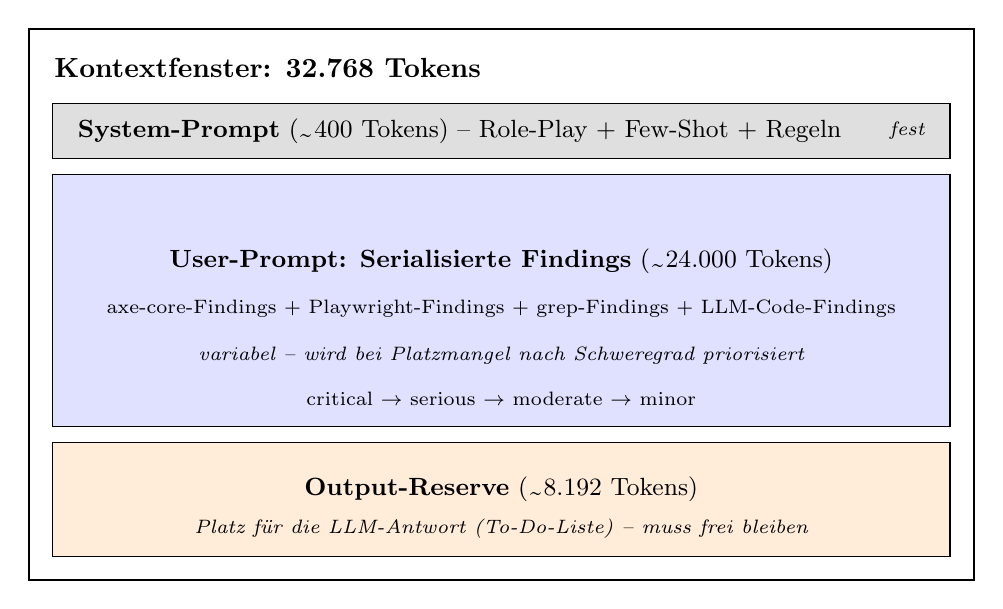
\begin{tikzpicture}
  % Gesamtrahmen
  \draw[thick] (0,0) rectangle (12,7);
  \node[anchor=north west, font=\bfseries] at (0.2,6.75) {Kontextfenster: 32.768 Tokens};

  % System-Prompt (oben, klein)
  \fill[gray!25] (0.3,5.35) rectangle (11.7,6.05);
  \draw (0.3,5.35) rectangle (11.7,6.05);
  \node[anchor=west, font=\small] at (0.5,5.7) {\textbf{System-Prompt} (\texttildelow{}400 Tokens) -- Role-Play + Few-Shot + Regeln};
  \node[anchor=east, font=\scriptsize\itshape] at (11.5,5.7) {fest};

  % Findings (Mitte, groß)
  \fill[blue!12] (0.3,1.95) rectangle (11.7,5.15);
  \draw (0.3,1.95) rectangle (11.7,5.15);
  \node[anchor=center, font=\small] at (6,4.05) {\textbf{User-Prompt: Serialisierte Findings} (\texttildelow{}24.000 Tokens)};
  \node[anchor=center, font=\scriptsize] at (6,3.45) {axe-core-Findings + Playwright-Findings + grep-Findings + LLM-Code-Findings};
  \node[anchor=center, font=\scriptsize\itshape] at (6,2.85) {variabel -- wird bei Platzmangel nach Schweregrad priorisiert};
  \node[anchor=center, font=\scriptsize] at (6,2.3) {critical $\rightarrow$ serious $\rightarrow$ moderate $\rightarrow$ minor};

  % Output-Reserve (unten)
  \fill[orange!15] (0.3,0.3) rectangle (11.7,1.75);
  \draw (0.3,0.3) rectangle (11.7,1.75);
  \node[anchor=center, font=\small] at (6,1.15) {\textbf{Output-Reserve} (\texttildelow{}8.192 Tokens)};
  \node[anchor=center, font=\scriptsize\itshape] at (6,0.65) {Platz f\"ur die LLM-Antwort (To-Do-Liste) -- muss frei bleiben};
\end{tikzpicture}

\caption[Aufteilung des Token-Budgets]{Aufteilung des Kontextfensters (32.768 Tokens) in drei Bereiche: System-Prompt (fest), serialisierte Findings (variabel, nach Schweregrad priorisiert) und Output-Reserve (fest). Vgl. Abschnitt~\ref{sec:kontextualisierung}.\protect\footnote{Eigene Abbildung}}
\label{fig:tokenbudget}
\end{figure}


\clearpage

\anhang{Screenshots der Testanwendung (test-12-Suite)}

\begin{figure}[htbp]
\centering
\includegraphics[width=0.95\textwidth]{graphics/test12-screen1.png}
\caption{Screenshot 1 der test-12-Suite}
\label{fig:test12_screen1}
\end{figure}

\begin{figure}[htbp]
\centering
\includegraphics[width=0.95\textwidth]{graphics/test12-screen2.png}
\caption{Screenshot 2 der test-12-Suite}
\label{fig:test12_screen2}
\end{figure}

\clearpage

\anhang{Accessibility-Verstöße der Testanwendung und zugehörige Prüfquellen (test-12-Suite)}

\begin{table}[htbp]
\centering
\setlength{\tabcolsep}{3.5pt}
\renewcommand{\arraystretch}{1.2}
\caption{Accessibility-Verstöße der Testanwendung und zugehörige Prüfquellen}
\begin{tabular}{|c|p{5.8cm}|c|p{4.2cm}|c|}
\hline
\textbf{\#} & \textbf{Violation} & \textbf{Kategorie} & \textbf{Erwartende Quelle} & \textbf{WCAG} \\
\hline
1 & \texttt{<img>} ohne alt-Attribut & syntaktisch & axe-core & 1.1.1 \\
\hline
2 & \texttt{<button>} ohne sichtbaren Text und ohne aria-label & syntaktisch & axe-core & 4.1.2 \\
\hline
3 & Formularfeld ohne \texttt{<label>} & syntaktisch & axe-core & 1.3.1 \\
\hline
4 & Kontrastverhältnis $< 4.5:1$ (Text auf Hintergrund) & layout & axe-core & 1.4.3 \\
\hline
5 & Fokus-Outline via CSS entfernt (\texttt{outline: none}) & layout & axe-core + Playwright & 2.4.7 \\
\hline
6 & onClick-Handler ohne onKeyDown-Pendant & semantisch & grep + LLM-Codeanalyse & 2.1.1 \\
\hline
7 & \texttt{role="button"} auf \texttt{<div>} ohne tabIndex & semantisch & axe-core + grep + LLM-Codeanalyse & 4.1.2 \\
\hline
8 & Modaler Dialog ohne Fokus-Trap & semantisch & Playwright & 2.1.2 \\
\hline
9 & Skip-Link fehlt & semantisch & Playwright & 2.4.1 \\
\hline
10 & \texttt{aria-hidden="true"} auf fokussierbarem Element & syntaktisch & axe-core & 4.1.2 \\
\hline
11 & Reihenfolge im DOM weicht von visueller Reihenfolge ab & semantisch & axe-core & 1.3.2 \\
\hline
12 & Interaktives Element zu klein ($<24\times24$px) & layout & grep + LLM-Codeanalyse & 2.5.8 \\
\hline
\end{tabular}
\label{tab:accessibility_verstoesse}
\end{table}

\clearpage

\anhang{Erkennungsrate der Violations im Proof of Concept (test-12-Suite)}

\begin{table}[htbp]
\centering
\setlength{\tabcolsep}{3.5pt}
\renewcommand{\arraystretch}{1.2}
\caption{Erkennungsrate der Violations im Proof of Concept}
\resizebox{\textwidth}{!}{%
\begin{tabular}{|c|p{5cm}|c|p{2.6cm}|c|p{2.8cm}|}
\hline
\textbf{\#} & \textbf{Violation} & \textbf{Erkannt (\checkmark/$\times$)} & \textbf{Tatsächliche Quelle} & \textbf{False Positive} & \textbf{Anmerkung} \\
\hline
1 & \texttt{<img>} ohne alt-Attribut & \checkmark & axe-core & - & Alle Modelle \\
\hline
2 & \texttt{<button>} ohne \texttt{aria-label} & \checkmark & LLM-Detektor & - & Nur 14b/32b; 7b miss \\
\hline
3 & Formularfeld ohne \texttt{<label>} & \checkmark & axe-core + grep & - & Alle Modelle \\
\hline
4 & Kontrastverhältnis $< 4.5:1$ & \checkmark & axe-core & - & 2 axe-Findings (nav + submit) \\
\hline
5 & Fokus-Outline entfernt (\texttt{outline: none}) & \checkmark & axe-core + Playwright & - & Alle Modelle \\
\hline
6 & onClick ohne onKeyDown & \checkmark & grep & - & Alle Modelle \\
\hline
7 & \texttt{role="button"} auf \texttt{<div>} ohne tabIndex & \checkmark & axe-core + grep & - & Alle Modelle \\
\hline
8 & Modal ohne Fokus-Trap & \checkmark & LLM-Detektor & - & Playwright-Check greift nicht; nur mit LLM \\
\hline
9 & Skip-Link fehlt & \checkmark & Playwright & - & Alle Modelle \\
\hline
10 & \texttt{aria-hidden="true"} auf fokussierbarem Element & \checkmark & axe-core & - & 7b lässt es gelegentlich weg \\
\hline
11 & DOM-Reihenfolge vs. visuelle Reihenfolge & \checkmark & LLM-Detektor & - & Nur 32b konsistent; 14b instabil \\
\hline
12 & Interaktives Element zu klein ($<24\times24$\,px) & \checkmark & LLM-Detektor & - & 7b instabil; 14b/32b konsistent \\
\hline
\end{tabular}
}%
\label{tab:erkennungsrate_poc}
\end{table}

\clearpage

\anhang{Bewertungsskala für die Empfehlungsqualität der LLM-Ausgaben (test-12-Suite)}

\begin{table}[htbp]
\centering
\setlength{\tabcolsep}{3.5pt}
\renewcommand{\arraystretch}{1.2}
\caption{Bewertungsskala für die Empfehlungsqualität der LLM-Ausgaben}
\begin{tabular}{|c|p{2.8cm}|p{7.2cm}|}
\hline
\textbf{Stufe} & \textbf{Bezeichnung} & \textbf{Kriterium} \\
\hline
2 & Konkret & Enthält Dateiname, Zeilennummer und einen konkreten Fix-Vorschlag (z.\,B. \texttt{aria-label="..."}). \\
\hline
1 & Teilweise & Enthält den richtigen Fix-Typ, jedoch ohne konkreten Codekontext (z.\,B. \glqq{}Füge ein aria-label hinzu\grqq). \\
\hline
0 & Generisch & Beschreibt lediglich das Problem, ohne einen umsetzbaren Lösungsvorschlag. \\
\hline
\end{tabular}
\label{tab:bewertungsskala_empfehlungen}
\end{table}

\clearpage
\anhang{Bewertung der Empfehlungsqualität pro Violation (test-12-Suite)}

\begin{table}[htbp]
\centering
\setlength{\tabcolsep}{3.5pt}
\renewcommand{\arraystretch}{1.2}
\caption{Bewertung der Empfehlungsqualität pro Violation}
\begin{tabular}{|c|p{4.8cm}|c|p{5.2cm}|}
\hline
\textbf{\#} & \textbf{Violation} & \textbf{Stufe (0--2)} & \textbf{Anmerkung (qwen3:32b)} \\
\hline
1 & \texttt{<img>} ohne alt-Attribut & 2 & Datei App.tsx:37, konkreter \texttt{alt}-Text angegeben \\
\hline
2 & \texttt{<button>} ohne \texttt{aria-label} & 2 & \texttt{aria-label}-Wert mit sprechendem Text vorgeschlagen \\
\hline
3 & Formularfeld ohne \texttt{<label>} & 2 & \texttt{label} + \texttt{htmlFor} + \texttt{id} vollständig ausgearbeitet \\
\hline
4 & Kontrastverhältnis $< 4.5:1$ & 2 & CSS-Regel mit konkreten Hex-Farben je betroffener Klasse \\
\hline
5 & Fokus-Outline entfernt (\texttt{outline: none}) & 2 & CSS-Klasse mit \texttt{outline: 2px solid} als Ersatz \\
\hline
6 & onClick ohne onKeyDown & 1 & \texttt{onKeyDown}-Muster korrekt, aber generisch; kein Dateikontext \\
\hline
7 & \texttt{role="button"} auf \texttt{<div>} ohne tabIndex & 2 & \texttt{tabIndex=\{0\}} + \texttt{onKeyDown} JSX-Snippet mit Kontext \\
\hline
8 & Modal ohne Fokus-Trap & 2 & Vollständiger \texttt{useEffect}-Fokus-Trap mit Shift+Tab-Logik \\
\hline
9 & Skip-Link fehlt & 2 & \texttt{<a href="\#main-content">}-Snippet mit CSS-Klasse \\
\hline
10 & \texttt{aria-hidden="true"} auf fokussierbarem Element & 2 & Korrektur (\texttt{aria-hidden} entfernen oder \texttt{tabIndex=\{-1\}}) mit Kontext \\
\hline
11 & DOM-Reihenfolge vs. visuelle Reihenfolge & 2 & CSS \texttt{order}-Property als Lösung; DOM-Reihenfolge erhalten \\
\hline
12 & Interaktives Element zu klein ($<24\times24$\,px) & 2 & CSS \texttt{width}/\texttt{height} auf 24\,px mit Klasse \texttt{.btn-tiny} \\
\hline
\end{tabular}
\label{tab:empfehlungsqualitaet}
\end{table}

\clearpage
\anhang{Recall-Matrix: Violation × Bedingung (test-12-Suite)}\label{app:recall_matrix}

\begin{table}[htbp]
\centering
\setlength{\tabcolsep}{4pt}
\renewcommand{\arraystretch}{1.25}
\caption[Recall-Matrix aller Violations je Bedingung]{Erkennungsstatus je Violation und Bedingung. \checkmark~=~konsistent erkannt; $\sim$~=~instabil (nur in einigen Runs); $\times$~=~nicht erkannt. Basis: test-12, jeweils 10~Runs.}
\resizebox{\textwidth}{!}{%
\begin{tabular}{|c|p{5.2cm}|c|c|c|c|c|}
\hline
\textbf{\#} & \textbf{Violation} & \textbf{Baseline} & \textbf{+\,7b} & \textbf{+\,14b} & \textbf{+\,32b} & \textbf{LLM-exklusiv} \\
\hline
1  & \texttt{<img>} ohne alt-Attribut                            & \checkmark & \checkmark & \checkmark & \checkmark & \\
\hline
2  & \texttt{<button>} ohne \texttt{aria-label} (Icon-Button)    & $\times$   & $\times$   & \checkmark & \checkmark & \checkmark \\
\hline
3  & Formularfeld ohne \texttt{<label>}                          & \checkmark & \checkmark & \checkmark & \checkmark & \\
\hline
4  & Kontrastverhältnis $<4.5:1$                                 & \checkmark & \checkmark & \checkmark & \checkmark & \\
\hline
5  & Fokus-Outline entfernt (\texttt{outline: none})             & \checkmark & \checkmark & \checkmark & \checkmark & \\
\hline
6  & onClick ohne onKeyDown                                      & \checkmark & \checkmark & \checkmark & \checkmark & \\
\hline
7  & \texttt{role="button"} auf \texttt{<div>} ohne tabIndex     & \checkmark & \checkmark & \checkmark & \checkmark & \\
\hline
8  & Modaler Dialog ohne Fokus-Trap                              & $\times$   & \checkmark & \checkmark & \checkmark & \checkmark \\
\hline
9  & Skip-Link fehlt                                             & \checkmark & \checkmark & \checkmark & \checkmark & \\
\hline
10 & \texttt{aria-hidden="true"} auf fokussierbarem Element      & \checkmark & $\sim$     & \checkmark & \checkmark & \\
\hline
11 & DOM-Reihenfolge weicht von visueller Reihenfolge ab         & $\times$   & $\times$   & $\sim$     & \checkmark & \checkmark \\
\hline
12 & Interaktives Element zu klein ($<24\times24$\,px)           & $\times$   & $\sim$     & \checkmark & \checkmark & \checkmark \\
\hline
\multicolumn{2}{|c|}{\textbf{Recall}} & \textbf{8\,/\,12} & \textbf{9\,/\,12} & \textbf{11\,/\,12} & \textbf{11--12\,/\,12} & 4~Violations \\
\hline
\end{tabular}
}%
\label{tab:recall_matrix}
\end{table}

\clearpage
\anhang{Rohdaten: alle 30 Benchmark-Runs (test-12-Suite)}\label{app:rohdaten}

\begin{table}[htbp]
\centering
\setlength{\tabcolsep}{3pt}
\renewcommand{\arraystretch}{1.1}
\caption[Rohdaten aller 30 Benchmark-Runs]{Vollständige Messdaten der 30 Pipeline-Durchläufe (test-12-Suite). LLM-Det.~=~Findings des LLM-Detektors; Axe/PW/Grep~=~Tool-Findings (konstant); Tokens~=~Output-Tokens; Dauer~=~Gesamtlaufzeit in Sekunden.}
\small
\resizebox{\textwidth}{!}{%
\begin{tabular}{|c|l|c|c|c|c|c|c|c|}
\hline
\textbf{Run} & \textbf{Modell} & \textbf{LLM-Det.} & \textbf{Axe} & \textbf{PW} & \textbf{Grep} & \textbf{Gesamt} & \textbf{Tokens} & \textbf{Dauer\,(s)} \\
\hline
01 & qwen2.5-coder:7b     & 11 & 4 & 2 & 6 & 23 &  6144 &  112 \\
02 & qwen2.5-coder:7b     & 11 & 4 & 2 & 6 & 23 &  6144 &  134 \\
03 & qwen2.5-coder:7b     & 11 & 4 & 2 & 6 & 23 &  6144 &  139 \\
04 & qwen2.5-coder:7b     &  4 & 4 & 2 & 6 & 16 &  2448 &   53 \\
05 & qwen2.5-coder:7b     & 10 & 4 & 2 & 6 & 22 &  6144 &  133 \\
06 & qwen2.5-coder:7b     & 16 & 4 & 2 & 6 & 28 &  3132 &   76 \\
07 & qwen2.5-coder:7b     & 14 & 4 & 2 & 6 & 26 &  2744 &   65 \\
08 & qwen2.5-coder:7b     &  9 & 4 & 2 & 6 & 21 &  6144 &  137 \\
09 & qwen2.5-coder:7b     & 14 & 4 & 2 & 6 & 26 &  3108 &   71 \\
10 & qwen2.5-coder:7b     & 11 & 4 & 2 & 6 & 23 &  2179 &   51 \\
\hline
11 & qwen2.5-coder:14b    & 23 & 4 & 2 & 6 & 35 &  3090 &  149 \\
12 & qwen2.5-coder:14b    & 23 & 4 & 2 & 6 & 35 &  6144 &  285 \\
13 & qwen2.5-coder:14b    & 23 & 4 & 2 & 6 & 35 &  5395 &  258 \\
14 & qwen2.5-coder:14b    & 23 & 4 & 2 & 6 & 35 &  6142 &  291 \\
15 & qwen2.5-coder:14b    & 23 & 4 & 2 & 6 & 35 &  5254 &  253 \\
16 & qwen2.5-coder:14b    & 22 & 4 & 2 & 6 & 34 &  6144 &  290 \\
17 & qwen2.5-coder:14b    & 23 & 4 & 2 & 6 & 35 &  5403 &  241 \\
18 & qwen2.5-coder:14b    & 23 & 4 & 2 & 6 & 35 &  2679 &  127 \\
19 & qwen2.5-coder:14b    & 22 & 4 & 2 & 6 & 34 &  6144 &  266 \\
20 & qwen2.5-coder:14b    & 23 & 4 & 2 & 6 & 35 &  6144 &  267 \\
\hline
21 & qwen3:32b            & 19 & 4 & 2 & 6 & 31 &  2846 &  290 \\
22 & qwen3:32b            & 20 & 4 & 2 & 6 & 32 &  3153 &  324 \\
23 & qwen3:32b            & 19 & 4 & 2 & 6 & 31 &  4233 &  440 \\
24 & qwen3:32b            & 19 & 4 & 2 & 6 & 31 &  2794 &  300 \\
25 & qwen3:32b            & 20 & 4 & 2 & 6 & 32 &  2908 &  312 \\
26 & qwen3:32b            & 19 & 4 & 2 & 6 & 31 &  2649 &  301 \\
27 & qwen3:32b            & 20 & 4 & 2 & 6 & 32 &  2963 &  311 \\
28 & qwen3:32b            & 20 & 4 & 2 & 6 & 32 &  4033 &  398 \\
29 & qwen3:32b            & 20 & 4 & 2 & 6 & 32 &  3191 &  321 \\
30 & qwen3:32b            & 19 & 4 & 2 & 6 & 31 &  6144 &  609 \\
\hline
\end{tabular}
}%
\label{tab:rohdaten_runs}
\end{table}

\clearpage
\anhang{Statistische Verteilung der LLM-Findings (alle 30 Runs, test-12-Suite)}\label{app:statistik_quantile}

\begin{table}[htbp]
\centering
\setlength{\tabcolsep}{4pt}
\renewcommand{\arraystretch}{1.2}
\caption[Quantilanalyse der LLM-Findings (alle 30 Runs)]{Quantilanalyse der LLM-Detektor-Findings über alle 30 Benchmark-Runs der test-12-Suite (3 Modelle $\times$ 10 Runs). Die Cluster-Struktur zeigt: 7b mit breiter Streuung (4--16), 14b und 32b mit engeren Ranges (22--23 bzw. 19--20).}
\begin{tabular}{|l|c|p{7cm}|}
\hline
\textbf{Quantil} & \textbf{Wert} & \textbf{Interpretation} \\
\hline
Min (0\,\%)     & 4 Findings  & absolutes Minimum (7b, Ausreißer) \\
\hline
Q1 (25\,\%)     & 11 Findings & 25\,\% der Runs liefern $\leq$ 11 Findings (7b-Cluster) \\
\hline
Median (50\,\%) & 19{,}5 Findings & typischer Wert; entspricht dem 32b-Cluster und unteren 14b-Bereich \\
\hline
Q3 (75\,\%)     & 22 Findings & 75\,\% der Runs liefern $\leq$ 22 Findings (14b-Bereich) \\
\hline
Max (100\,\%)   & 23 Findings & absolutes Maximum (14b, oberer Bereich) \\
\hline
IQR             & 11 Findings & Streuung der mittleren 50\,\% -- spiegelt Modell-Heterogenität wider \\
\hline
\end{tabular}
\label{tab:statistik_quantile}
\end{table}

\clearpage
\anhang{Modell-Leistungsvergleich: test-12-Suite Zusammenfassung}\label{app:modell_summary}

\begin{table}[htbp]
\centering
\setlength{\tabcolsep}{4pt}
\renewcommand{\arraystretch}{1.25}
\caption[Modell-Leistungsvergleich (alle Metriken)]{Zusammenfassung aller Leistungsmetriken für die drei evaluierten Modelle (test-12-Suite, je $n=10$ Runs). $\sigma$~=~Standardabweichung der LLM-Detektor-Findings über 10~Runs.}
\resizebox{\textwidth}{!}{%
\begin{tabular}{|l|c|c|c|}
\hline
\textbf{Metrik} & \textbf{qwen2.5-coder:7b} & \textbf{qwen2.5-coder:14b} & \textbf{qwen3:32b} \\
\hline
Recall (Ø über Runs)              & $\sim$75\,\%     & $\sim$91{,}7\,\%  & 91{,}7--100\,\% \\
LLM-Detektor-Findings (Ø)         & 11{,}1           & 22{,}8             & 19{,}5 \\
LLM-Detektor-Findings (Min--Max)  & 4--16            & 22--23             & 19--20 \\
Konsistenz $\sigma$               & 3{,}28           & 0{,}42             & 0{,}53 \\
Priorisierung                     & Fehlerhaft       & Verbessert         & Korrekt \\
Fix-Qualität (Stufe)              & 0--1             & 1                  & 1--2 \\
Gesamtlaufzeit (Ø)                & 231\,s           & 420\,s             & 701\,s \\
LLM-Detektor-Laufzeit (Ø)        & 139\,s           & 231\,s             & 374\,s \\
LLM-Priorisierung (Ø)            & 92\,s            & 189\,s             & 327\,s \\
Output-Tokens (Ø)                 & 4{,}433          & 5{,}254            & 3{,}491 \\
Token-Limit-Erreicht              & Selten           & Selten             & Selten \\
Parsing-Erfolg                    & 100\,\%          & 100\,\%            & 100\,\% \\
Eignung BITV-Einsatz              & Nicht geeignet   & Empfohlen          & Empfohlen (Forsch.) \\
\hline
\end{tabular}
}%
\label{tab:modell_summary}
\end{table}

\clearpage
\anhang{Vergleich aller vier Modellkandidaten: test-12-Suite Evaluationsergebnisse}\label{app:modellvergleich_4}

\begin{table}[htbp]
\centering
\setlength{\tabcolsep}{4pt}
\renewcommand{\arraystretch}{1.25}
\caption[Vergleich aller vier Modellkandidaten]{Qualitative und quantitative Gegenüberstellung der vier in Kapitel~\ref{kap:4} eingeführten Modellkandidaten. Die ausgewiesenen Messwerte für 7b/14b/32b basieren ausschließlich auf der test-12-Suite. Für \texttt{deepseek-r1:70b} liegen im Rahmen dieser Arbeit keine Messwerte vor (ausstehend); die Evaluation ist als Folgeschritt geplant (vgl. Abschnitt~\ref{sec:eval_erweiterung}).}
\resizebox{\textwidth}{!}{%
\begin{tabular}{|l|c|c|c|}
\hline
\textbf{Metrik} & \textbf{qwen2.5-coder:7b} & \textbf{qwen2.5-coder:14b} & \textbf{qwen3:32b} \\
\hline
Modelltyp                   & Code          & Code          & Generalist \\
\hline
Parameter                   & 7B            & 14B           & 32B \\
\hline
Recall (test-12)            & $\sim$75\,\%  & $\sim$91{,}7\,\% & 91{,}7--100\,\% \\
\hline
LLM-Findings Ø         & 11{,}1 ± 3{,}28 & 22{,}8 ± 0{,}42 & 19{,}5 ± 0{,}53 \\
\hline
Konsistenz $\sigma$         & 3{,}28        & 0{,}42        & 0{,}53 \\
\hline
Priorisierungsqualität      & Fehlerhaft (invers) & Verbessert & Korrekt \\
\hline
Fix-Qualität (Stufe)        & 0--1          & 1             & 1--2 \\
\hline
Gesamtlaufzeit Ø            & 231\,s        & 420\,s        & 701\,s \\
\hline
Output-Tokens Ø             & 4\,433        & 5\,254        & 3\,491 \\
\hline
NFA-02-Konformität          & \checkmark    & \checkmark    & \checkmark \\
\hline
Eignung BITV-Einsatz        & Nicht geeignet & Empfohlen & Empfohlen (Forschung) \\
\hline
\end{tabular}
}%
\label{tab:modellvergleich_4}
\end{table}

\clearpage
\anhang{Einsatzempfehlungen nach Anwendungsszenario (test-12-Suite)}\label{app:einsatzempfehlungen}

\textbf{Leseanleitung:} Die nachfolgende Tabelle setzt die Evaluationsergebnisse aus Kapitel~\ref{kap:7} voraus und bezieht sich auf die test-12-Suite. \texttt{qwen2.5-coder:7b} erscheint in der Spalte \textit{Primär} ausschließlich in Szenarien, in denen \textbf{kein} BITV-/WCAG-konformes Ergebnis erforderlich ist (CI/CD-Rauchtest, Prototyp). Für jede rechtlich relevante Barrierefreiheitsprüfung gilt unverändert: \texttt{qwen2.5-coder:7b} ist aufgrund der nachgewiesenen inversen Priorisierung (vgl. Abschnitt~\ref{sec:prio_modellvergleich}) \textit{nicht geeignet}. Die Spalte \textit{Eignung BITV-Einsatz} in Anhang~\ref{tab:modell_summary} ist das übergeordnete Kriterium.

\begin{table}[htbp]
\centering
\setlength{\tabcolsep}{4pt}
\renewcommand{\arraystretch}{1.2}
\caption[Modellempfehlungen nach Anwendungsszenario]{Empfohlene Modellwahl in Abhängigkeit vom Einsatzkontext. Primär: bevorzugtes Modell; Sekundär: Alternative. Die Empfehlungen für 7b gelten ausschließlich für nicht-compliance-relevante Szenarien.}
\begin{tabular}{|p{5.0cm}|c|c|p{5.6cm}|}
\hline
\textbf{Szenario} & \textbf{Primär} & \textbf{Sekundär} & \textbf{Begründung} \\
\hline
CI/CD-Rauchtest (nicht compliance-relevant) & 7b & 14b & Schnellstes Feedback; inverse Priorisierung hier tolerierbar \\
\hline
Regulärer Entwicklungszyklus & 14b & 32b & Bester Kompromiss aus Recall, Priorisierung und Laufzeit \\
\hline
BITV-Compliance-Audit        & 14b & 32b & Recall~$\geq$~91{,}7\,\%, korrekte Priorisierung, NFA-02 erfüllt \\
\hline
Abnahmeprüfung / Endaudit    & 32b & 14b & Höchster Recall (100\,\%), $\sigma = 0{,}42$, Stufe-2-Fixes \\
\hline
Prototyp / MVP               & 7b  & -  & Schnelle Iteration; für finale Abnahme durch 14b/32b ersetzen \\
\hline
Enterprise-Deployment        & 14b & 32b & Produktionstaugliches Qualitätsniveau \\
\hline
\end{tabular}
\label{tab:einsatzempfehlungen}
\end{table}

\clearpage
\anhang{Detektor-Konsistenz über alle 30 Runs (test-12-Suite)}\label{app:detektor_konsistenz}

\begin{table}[htbp]
\centering
\setlength{\tabcolsep}{3pt}
\renewcommand{\arraystretch}{1.2}
\scriptsize
\caption[Detektor-Konsistenz über alle Runs]{Konsistenzanalyse der Detektoren über alle 30 Benchmark-Runs (test-12). Da axe-core, Playwright und grep vollständig deterministisch bleiben, wird die relevante Varianz auf Modellebene innerhalb des LLM-Detektors ausgewiesen.}
\resizebox{\textwidth}{!}{%
\begin{tabular}{|p{2.4cm}|p{0.8cm}|p{1.5cm}|p{1.2cm}|p{1.2cm}|p{1.7cm}|p{3.8cm}|}
\hline
\textbf{Detektor / Modell} & \textbf{Runs} & \textbf{Gesamt- findings} & \textbf{Ø pro Run} & \textbf{Min--Max} & \textbf{$\sigma^2$ / $\sigma$} & \textbf{Interpretation} \\
\hline
axe-core    & 30 & 120 & 4,0  & 4--4   & 0,00 / 0,00 & vollständig deterministisch \\
\hline
Playwright  & 30 & 60  & 2,0  & 2--2   & 0,00 / 0,00 & vollständig deterministisch \\
\hline
grep        & 30 & 180 & 6,0  & 6--6   & 0,00 / 0,00 & vollständig deterministisch \\
\hline
qwen2.5-coder:7b  & 10 & 111 & 11,1 & 4--16  & 9,69 / 3,11 & höchste Streuung \\
\hline
qwen2.5-coder:14b & 10 & 228 & 22,8 & 22--23 & 0,16 / 0,40 & hohe Konsistenz bei höchster Trefferzahl \\
\hline
qwen3:32b         & 10 & 195 & 19,5 & 19--20 & 0,25 / 0,50 & stabil, aber mit höherer Laufzeit \\
\hline
LLM-Detektor gesamt & 30 & 534 & 17,8 & 4--23 & modell\-abhängig & -- \\
\hline
\end{tabular}
}%
\label{tab:detektor_konsistenz}
\end{table}

Die Tabelle zeigt, dass die Unterschiede zwischen den Detektoren selbst methodisch kaum relevant sind: axe-core, Playwright und grep liefern über alle 30 Runs exakt konstante Ergebnisse. Die tatsächlich relevante Varianz entsteht ausschließlich innerhalb des \ac{LLM}-Detektors und dort vor allem durch die Modellwahl. \texttt{qwen2.5-coder:14b} weist mit $\sigma = 0{,}40$ die höchste Konsistenz bei zugleich höchster durchschnittlicher Fundzahl auf, während \texttt{qwen2.5-coder:7b} mit $\sigma = 3{,}11$ deutlich volatiler reagiert. \texttt{qwen3:32b} ist ebenfalls sehr stabil ($\sigma = 0{,}50$), erkauft diese Stabilität jedoch mit einer wesentlich höheren Laufzeit. Für die Interpretation der Gesamtpipeline ist daher nicht die Frage entscheidend, welcher Detektor variiert, sondern welches Modell im \ac{LLM}-Detektor eingesetzt wird.

\anhang{Effizienzmetriken und Kosten-Nutzen-Verhältnis (test-12-Suite)}\label{app:effizienz_metriken}

\begin{table}[htbp]
\centering
\setlength{\tabcolsep}{4pt}
\renewcommand{\arraystretch}{1.2}
\caption[Effizienzvergleich der Modelle]{Effizienzvergleich auf Basis der 30 Benchmark-Runs der test-12-Suite. \textit{LLM-Findings/s} bezieht sich auf LLM-Detektor-Findings pro Sekunde Gesamtlaufzeit.}
\resizebox{\textwidth}{!}{%
\begin{tabular}{|l|c|c|c|c|}
\hline
\textbf{Modell} & \textbf{LLM-Findings Ø} & \textbf{Gesamtlaufzeit Ø (s)} & \textbf{LLM-Findings/s} & \textbf{Zusatznutzen ggü. 7b} \\
\hline
qwen2.5-coder:7b  & 11{,}1 & 231 & 0{,}048 & Referenz \\
\hline
qwen2.5-coder:14b & 22{,}8 & 420 & 0{,}054 & +105\,\% bei +82\,\% Zeitaufwand \\
\hline
qwen3:32b         & 19{,}5 & 701 & 0{,}028 & +76\,\% bei +203\,\% Zeitaufwand \\
\hline
\end{tabular}
}%
\label{tab:effizienz_metriken}
\end{table}

\clearpage

\anhang{Token-Nutzung pro Modell: Input/Output (test-12-Suite)}\label{app:token_economy}

\begin{table}[htbp]
\centering
\setlength{\tabcolsep}{4pt}
\renewcommand{\arraystretch}{1.2}
\caption[Token-Nutzung pro Modell]{Durchschnittliche Token-Nutzung je Run und Modell auf Basis der test-12-Suite. Input-Tokens umfassen System-Prompt, serialisierte Findings und Konfigurationsparameter; Output-Tokens entsprechen der generierten Priorisierungsliste. Alle 7b- und 14b-Runs erreichten das Output-Limit von 3\,072 (Antwortabbruch); 32b-Runs lagen im Mittel bei 2\,979.}
\begin{tabular}{|l|c|c|c|}
\hline
\textbf{Modell} & \textbf{Input-Tokens Ø} & \textbf{Output-Tokens Ø} & \textbf{Truncation} \\
\hline
qwen2.5-coder:7b  & 3\,669 & 3\,072 & 10/10 Runs (100\,\%) \\
\hline
qwen2.5-coder:14b & 3\,947 & 3\,072 & 10/10 Runs (100\,\%) \\
\hline
qwen3:32b         & 4\,386 & 2\,979 &  6/10 Runs (60\,\%) \\
\hline
\multicolumn{4}{|l|}{\textit{Gesamt (30 Runs): Input $\approx$120\,400 / Output 91\,226 / Prompt $\approx$125\,800 Tokens}} \\
\hline
\end{tabular}
\label{tab:token_economy}
\end{table}

\anhang{Über-Detektion relativ zur Ground Truth (test-12-Suite)}\label{app:overdetection}

\begin{table}[htbp]
\centering
\setlength{\tabcolsep}{4pt}
\renewcommand{\arraystretch}{1.2}
\caption[Über-Detektion relativ zu 12 Ground-Truth-Violations]{Vergleich der durchschnittlichen Gesamtfindings pro Run mit der Ground Truth (12 Violations) auf Basis der test-12-Suite. Hohe Werte deuten auf zusätzliche Hinweise und/oder semantische Redundanzen hin.}
\resizebox{\textwidth}{!}{%
\begin{tabular}{|l|c|c|c|p{5.3cm}|}
\hline
\textbf{Modell} & \textbf{Gesamtfindings Ø} & \textbf{Ground Truth} & \textbf{Quote} & \textbf{Interpretation} \\
\hline
qwen2.5-coder:7b  & 22,3 & 12 & 186\,\% & moderater Überschuss; Recall-Gewinn begrenzt, Priorisierung instabil \\
\hline
qwen2.5-coder:14b & 31,8 & 12 & 265\,\% & deutlicher Überschuss; hoher Recall, jedoch erhöhte Redundanz \\
\hline
qwen3:32b         & 31,2 & 12 & 260\,\% & ähnlicher Überschuss wie 14b, aber mit höherer Konsistenz \\
\hline
\end{tabular}
}%
\label{tab:overdetection}
\end{table}

\clearpage
\anhang{CSV-Export der Benchmark-Rohdaten (test-12-Suite)}\label{app:csv_export}

Die Benchmark-Rohdaten wurden zusätzlich als CSV-Datei exportiert (\texttt{results\-/bench\-mark\-/summary.csv}). Tabelle~\ref{tab:csv_schema} dokumentiert das reale Spaltenschema, Tabelle~\ref{tab:csv_beispiel} zeigt exemplarische Zeilen (je ein Run pro Modell).

\begin{table}[htbp]
\centering
\setlength{\tabcolsep}{4pt}
\renewcommand{\arraystretch}{1.2}
\caption[CSV-Spaltenschema]{Spaltenschema des CSV-Exports \texttt{results/benchmark/summary.csv}.}
\resizebox{\textwidth}{!}{%
\begin{tabular}{|l|p{8.7cm}|}
\hline
\textbf{Spalte} & \textbf{Bedeutung} \\
\hline
model & Verwendetes Modell (z.\,B. qwen2.5-coder:14b) \\
\hline
suite & Testsuite (hier: test-12) \\
\hline
run & Laufnummer innerhalb einer Modellserie \\
\hline
success / parseSuccess & Pipeline-Erfolg und Parsing-Erfolg der Ausgabe \\
\hline
mustHaveCount / niceToHaveCount & Anzahl Must-have- bzw. Nice-to-have-Findings im finalen Report \\
\hline
durationMs & Gesamtlaufzeit der Pipeline in Millisekunden \\
\hline
promptTokens / outputTokens & Tatsächlich verwendete Prompt- und Output-Tokens \\
\hline
numPredict & Verwendetes Output-Token-Limit der Priorisierungsphase \\
\hline
Axe / Playwright / Grep / LLM & Anzahl erkannter Findings je Detektor \\
\hline
error & Fehlermeldung (leer bei erfolgreichem Run) \\
\hline
\end{tabular}
}%
\label{tab:csv_schema}
\end{table}

\begin{table}[htbp]
\centering
\setlength{\tabcolsep}{3.5pt}
\renewcommand{\arraystretch}{1.15}
\caption[Beispielzeilen aus dem CSV-Export]{Repräsentative Beispielzeilen aus \texttt{results/benchmark/summary.csv} (test-12-Suite; jeweils Run~01 pro Modell).}
\resizebox{\textwidth}{!}{%
\begin{tabular}{|l|c|c|c|c|c|c|c|c|c|c|c|}
\hline
\textbf{model} & \textbf{run} & \textbf{must} & \textbf{nice} & \textbf{LLM} & \textbf{Axe} & \textbf{PW} & \textbf{Grep} & \textbf{durationMs} & \textbf{prompt} & \textbf{output} & \textbf{parse} \\
\hline
qwen2.5-coder:7b  & 1 & 14 & 33 & 11 & 4 & 2 & 6 & 111817 & 4405 & 6144 & true \\
\hline
qwen2.5-coder:14b & 1 & 6 & 16 & 23 & 4 & 2 & 6 & 148920 & 5635 & 3090 & true \\
\hline
qwen3:32b         & 1 & 12 & 8 & 19 & 4 & 2 & 6 & 289630 & 5200 & 2846 & true \\
\hline
\end{tabular}
}%
\label{tab:csv_beispiel}
\end{table}